% siminos/CLE/CLE.tex
% $Author$ $Date$

                            \newif\ifdraft \newif\ifpaper
 \drafttrue\paperfalse      % draft version, commented
%\draftfalse\paperfalse     % final version, hyperlinks
%\draftfalse\papertrue      % final version, no hyperlinks, for printing
%%%%%%%%%%%%%%%%%%%%%%%%%%%%%%%%%%%%%%%%%%%%%%%%%%%%%%%%

% Predrag reorganized siminos/CLE/          2009-10-09
% Vaggelis created siminos/CLE/CLE.tex      2009-09-21
% Vaggelis created siminos/CLE              2009-02-05

\ifdraft
\documentclass[preprint,number,sort&compress]{elsarticle}
\else
\documentclass[final,number]{elsarticle}
\fi

\usepackage{amsmath,amsfonts,amssymb,amsbsy,amscd}
\usepackage{ifthen}
\usepackage{graphicx}
\usepackage[dvips]{color}
\usepackage[dvips,colorlinks]{hyperref}
\graphicspath{{../figs/}{../Fig/}}  %% directories with graphics files
\input ../inputs/def        % TEMPORARY
\input inputs/defsCLE.tex   % eventualy merge used commanDs into inputs/defsCLE.tex

% Use the next command to get Bibliography header appear. The problem is a conflict
% between elsarticle and amsref over \bibsection command.
 \renewcommand\bibname{References}
 \newcommand\bibsection{%
   \section*{\bibname\markright{\MakeUppercase{\bibname}}}}

\begin{document}
\journal{Physica D}
\begin{frontmatter}

			\title{
Continuous symmetry reduction and return maps for higher-dimensional flows
			}
% Continuous symmetry reduction and return maps for high dimensional flows
% Continuous symmetry reduced return maps for high dimensional flows
% Returm maps of high dimensional flows with continuous symmetry:
%                                           I. Symmetry reduction
% Towards continuous symmetry reduction in high dimensional flows
\author{Evangelos Siminos}
\ead{siminos@gatech.edu}
\author{Predrag Cvitanovi\'c}
\address{Center for Nonlinear Science,
School of Physics, Georgia Institute of Technology,
Atlanta, GA 30332-0430}
%\homepage[]{Your web page}
%\thanks{}
%\altaffiliation{}


\date{\today}

        \begin{abstract}
\input abstract
        \end{abstract}

\begin{keyword}
continuous symmetry reduction,
relative equilibria,
relative periodic orbits,
return maps,
slices,
moving frames,
Hilbert polynomial bases
\PACS 05.45.-a \sep 47.27.ed \sep 42.65.Sf
% 05.45.-a 	Nonlinear dynamics and chaos
% 05.45.Jn 	High-dimensional chaos
% 47.10.Fg 	Dynamical systems methods (in Fluid Mechanics)
% 47.27.ed 	Dynamical systems approaches (turbulent flows)
% 47.52.+j 	Chaos in fluid dynamics
% 42.65.Sf 	Dynamics of nonlinear optical systems; optical instabilities,
% 		optical chaos and complexity, and optical spatio-temporal dynamics
\end{keyword}
\end{frontmatter}

\section{\label{s:intro} Introduction}
    \PC{please keep improving abstract, intro and conclusions at each proofreading.
    \\
    remove PC\{\} and PCedit\{\} after you have accepted/edited them}
    \input intro

% \section{\label{s:symDyn} Symmetries of dynamical systems}
    \input symDyn

% \subsection{\label{s:introCLE} An example: \CLe}
    % introducing CLe
% from siminos/thesis/lasersSym.tex

\CLe\ were introduced by Gibbon and McGuinness\rf{GibMcCLE82} as a low-dimensional model
of baroclinic instability in the atmosphere.
As the name suggests they turned out to be a complex generalization
of Lorenz equations\rf{lorenz}:
\beq
\index{Complex Lorenz equations}
\begin{split}
 \dot{x} &=-\sigma x+ \sigma y \cont
 \dot{y} &=(\rLor-z)x-a y \cont
 \dot{z} &= \frac{1}{2}\left(x y^*+x^*y\right)-b z\,,
 \label{eq:CLe}
\end{split}
\eeq
where now $x,y$ are complex variables, $z$ is real, while the
parameters $\sigma,\,b$ are real and $\rLor=\RerCLor+i
\ImrCLor$, $a=1-i e$ are complex.
In all numerical examples
that follow, the parameters will be set to the Lorenz values
$\RerCLor=28,\, b=8/3,\, \sigma=10,\, a=1$, unless explicitly
stated otherwise.

Ning and Haken\rf{NingHakenCLE90} have shown
that equations isomorphic to \CLe\ also appear as a
truncation of Maxwell-Bloch equations describing a single
mode, detuned, ring laser.
%with $x,y$ and $z$
%proportional to electric field, polarization and population inversion, respectively.
They set $e+\ImrCLor=0$ so that a detuned
\eqv\ exists.
    \ES{This assumption is questionable unless it
is forced by the physics of the problem, which I cannot
follow very well. It leads to non-generic bifurcation
behavior, while one would like a model of a physical system
to be robust under perturbations (of the model). Furthermore,
the fact that the Hopf cycle in the general case is an
$\SOn{2}$-orbit has gone unnoticed. The \reqv\ can be
interpreted as an \eqv\ in a rotating frame and the measured
electric field of the laser would be the same in both cases.
    }
Bakasov and Abraham\rf{BakasovAbraham93} criticize this
choice as being ``degenerate'' and show that one can use
\CLe\ with $\ImrCLor=0$ and $e \neq 0$ to describe detuned lasers.
As we explain in \refsect{sec:Eqv0}, the choice of Ning and
Haken leads to non-generic bifurcations.


% \section{\label{s:symSol} Solutions of systems with continuous symmetry}
   % siminos/CLE/symSol.tex
% $Author$ $Date$

\section{\label{s:symSol} Symmetries of solutions}

In order to explore the implications of equivariance for the
solutions of dynamical equations,  we start by examining the
way a compact Lie group acts on \statesp\ \pS. The
\emph{group orbit} or the \emph{$\Group$-orbit} of the point
$\ssp \in \pS$ is the set
\beq
    \pS_\ssp = \{\LieEl\,\ssp \mid \LieEl \in {\Group}\}
\ee{GroupOrb}
of all \statesp\ points into which $\ssp$ is mapped under the
action of $\Group$.
The \emph{symmetry} $\stab{\ssp}$ (\emph{isotropy} or
\emph{stabilizer} group) of a \statesp\ point $\ssp$ is the
largest subgroup of $\Group$
\beq
\stab{\ssp} =\{\LieEl \in \Group: \LieEl \ssp = \ssp \}
\ee{def:isotr}
that leaves $\ssp$ fixed.
The \emph{symmetry} $\stab{X}$ of a set $\pS_X \in \pS$ is
the largest subgroup  of $\Group$ that leaves $\pS_X$
invariant as a set:
\[
	\stab{X}= \{\LieEl: \LieEl \, \pS_X = \pS_X\}
\,.
\]
If $\stab{p}$ is a symmetry, intrinsic properties of a
solution $\pS_p$ (such as \eqv\ or a cycle stability
eigenvalues, period, Floquet multipliers) evaluated anywhere
along its $\stab{p}$-orbit are the same. A symmetry thus
reduces the number of inequivalent solutions. So we also need
to describe the symmetry of a \emph{solution}, as opposed to
\refeq{eq:equivFinite}, the symmetry of the \emph{system}.

The \emph{\fixedsp} $\Fix{\Subgroup}$ of a subgroup
$\Subgroup\subset\Group$ is the subspace of $\pS$ containing
all fixed points of $\Subgroup$:
\[
	\Fix{\Subgroup}=
      \{\ssp\in\pS,\,\LieEl\in\Subgroup \,|\,
        \LieEl \ssp = \ssp \}
\,.
\]
The physical importance of \fixedsp s lies in the fact that
they are invariant under $\Group$-equivariant
dynamics\rf{golubitsky2002sp},
\[
 f^\tau\left(\Fix{\Subgroup}\right)\subseteq \Fix{\Subgroup}
\]
for all times $\tau$. Therefore if $\ssp(\tau)$ is a solution
of an equivariant ODE then its symmetry
$\stab{\ssp(\tau)}=\stab{\ssp(0)}$ is preserved for for all
times.

In contrast to \emph{\eqv} solutions that satisfy
$f^\tau(\ssp)  =  \ssp$, \emph{\reqva} satisfy
$f^\tau(\ssp) = \LieEl( \tau) \, \ssp$ for any $\tau$,
see \reffig{f:MeanVelocityFrame}. In
a co-moving frame moving along the group orbit
with velocity $\vel(\ssp) = \velRel \cdot \groupTan(\ssp)$,
    \ES{define $\groupTan$ in symmetry section, choose
    a prettier symbol. {\bf PC:} I see it coming; you will
    make it all look Greek to me. {\bf ES:} Well, unless
	you want to change time to $\tau$ we have to change
	group tangent. {\bf PC:} I do call time $\tau$ in
    continuous.tex .}
the \reqv\ appears as an \eqv.

A {\em \rpo}is an orbit $\pS_p$ for
which the initial point exactly recurs
    \index{periodic!orbit!relative}\index{relative!periodic orbit}
\beq
\ssp_p (0) = \LieEl_p \ssp_p (\period{p} )
    \,,\qquad
\ssp_p (\tau) \in \pS_p
    \,,
\label{RPOrelper1}
\eeq
at a fixed {\em relative period} $\period{p}$, but shifted by
a fixed group action ${\LieEl_p}$ which brings the endpoint
$\ssp_p (\period{p} ) $ back into the initial point $\ssp_p
(0) $, see \reffig{f:rpo}\,(b). The group action ${\LieEl_p}=
\LieEl_p(\gSpace)$ parameters $\gSpace_p =
(\gSpace_1,\gSpace_2,\cdots\gSpace_N)$ will be referred to as
``phases,'' or ``shifts.'' For dynamical systems with only
continuous (no discrete) symmetries, the parameters
$\{t,\gSpace_1,\cdots,\gSpace_N\}$ are real numbers, ratios
$\pi/\gSpace_j$ are almost never rational, and the likelihood
of closing into a {\po} is {zero}. Thus the trajectory
of \rpo\ generically sweeps out the group orbit ergodically.
%
%%%%%%%%%%%%%%%%%%%%%%%%%%%%%%%%%%%%%%%%%%%%%%%%%%%%%%%%%%%%%%%%
% hand-drawn in dasbuch/book/FigSrc/xfig/rpo.fig
\begin{figure}[ht]
 (a)\includegraphics[width=0.40\textwidth]{../Fig/reqv.eps}
~(b)\includegraphics[width=0.40\textwidth]{../Fig/rpo.eps}
\caption{
(a) A {\em \reqv\ orbit} starts out at some point $\ssp(0)$,
with the dynamical flow field $\vel(\ssp) = \velRel \cdot
\groupTan(\ssp)$ pointing along the group tangent space. For
the $\SOn{2}$ symmetry depicted here, the flow traces out the
group orbit of $\ssp(0)$ in time $\period{}=2\pi/\velRel$.
An
{\em \eqv} lives either in the $\Fix{\Group}$ subspace
($x_3$ axis in this sketch), or on a group orbit as the one
depicted here, but with zero angular velocity $\velRel$. In
that case the circle (in general, $N$-torus) depicts a
continuous family of fixed \eqva, related only by the group
action.
(b) A {\em \rpo} starts out at $\ssp(0)$ with the dynamical $\vel$ and
group tangent $\groupTan$ flows pointing in different
directions, and returns to the group orbit of $\ssp(0)$ after
time $\period{p}$ at $\ssp(\period{p})=\LieEl_p \ssp (0)$, a
rotation of the initial point by $\LieEl_p$.
}
\label{f:rpo}
\end{figure}
%%%%%%%%%%%%%%%%%%%%%%%%%%%%%%%%%%%%%%%%%%%%%%%%%%%%%%%%%%%%%%%%%%

A \emph{\rpo} is periodic in its
mean velocity $\velRel_p=\gSpace_p/\period{p}$ co-rotating
frame (see \reffig{f:MeanVelocityFrame}), but in the
stationary frame its trajectory is quasiperiodic.
A co-moving
frame is helpful in visualizing a single `relative' orbit,
but useless for viewing collections of orbits, as each one
drifts with its own angular velocity. Visualization of all
\rpo s as \po s we attain only by global\marginpar{explain global vs
local in intro. It is not really global.} symmetry reduction,
to be undertaken in the following.

%
%%%%%%%%%%%%%%%%%%%%%%%%%%%%%%%%%%%%%%%%%%%%%%%%%%%%%%%%%%%%%%%%
% from siminos/rpo_ks/arxiv-v2/figs
\begin{figure}[ht]
(a)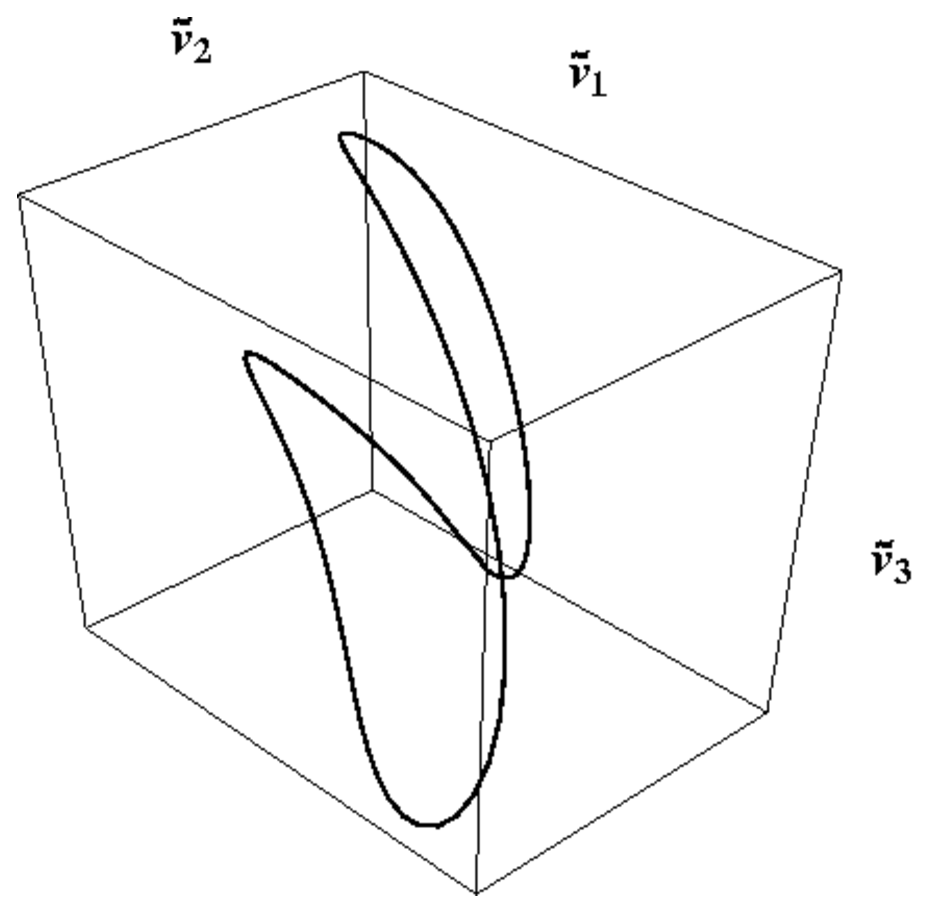
\includegraphics[width=0.40\textwidth, clip=true]
                    {../figs/ks22rpo033.50_04.045E2.eps}
~(b)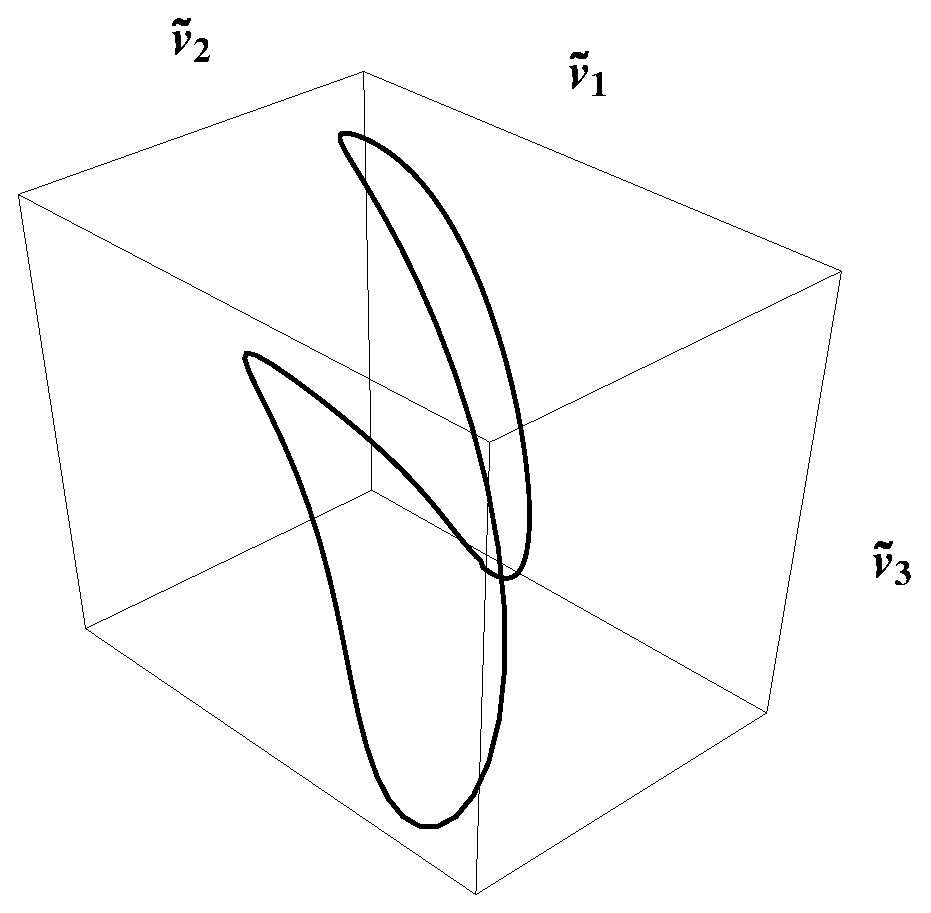
\includegraphics[width=0.40\textwidth, clip=true]
                     {../figs/ks22rpo033.50_04.045E2CM.eps}
\caption{
 A \rpo\ of Kuramoto-Sivashinsky flow, traced for four periods
 $\period{p}$ and projected on
 (a) the stationary \statesp\ coordinate frame
 $\{v_1,v_2,v_3\}$;
 (b) the co-moving $\{\tilde{v}_1,\tilde{v}_2,\tilde{v}_3\}$
 coordinate frame, moving with the mean velocity
 $\velRel_p=\gSpace_p/\period{p}$.
\hfill (from \refref{SCD07})
}
\label{f:MeanVelocityFrame}
\end{figure}
%%%%%%%%%%%%%%%%%%%%%%%%%%%%%%%%%%%%%%%%%%%%%%%%%%%%%%%%%%%%%%%%%%

   % siminos/CLE/CLEsols.tex
% $Author$ $Date$

\subsection{\label{s:CLEsols} An example: Solutions of \cLe}

In the case of {\cLe}  the origin \EQV{0} is an \eqv\ of
\refeq{eq:CLe} for any value of the parameters. As shown in
\refref{FowlerCLE82} it is stable for $0<\RerCLor<\rho_{1c}$
and unstable for $\rho_{1c}<\RerCLor$, where
\beq
	\rho_{1c} = 1 + \frac{(e+\ImrCLor)(e-\sigma \ImrCLor)}{(\sigma+1)^2}\,.
\eeq
At bifurcation a pair of eigenvalues crosses the imaginary
axis with imaginary part:
\beq
	\omega_c = \frac{\sigma (e + \ImrCLor)}{\sigma+1}\,.
	\label{eq:omegaCLE}
\eeq
and a \emph{relative equilibrium} \REQV{}{1} is born. For
$e+\ImrCLor=0$ the relative equilibrium degenerates to an
\SOn{2}-orbit of \eqva\rf{FowlerCLE82}, since $\omega_c =0$.
Ning and Haken\rf{NingHakenCLE90} and Zeghlache and
Mandel\rf{ZeMa85} use equations isomorphic to \cLe\ with
$e+\ImrCLor=0$ in their studies of detuned ring lasers.
Existence of a \reqv\ in a system with \SOn{2} symmetry is
the generic situation, so here we will use Bakasov and
Abraham\rf{BakasovAbraham93} choice $\ImrCLor=0$ and $e \neq
0$.

As $\RerCLor$ is increased,  a secondary bifurcation from
\REQV{}{1} is expected, according to Krupa's
theorem\rf{Krupa90}, to result in \emph{\rpo s} that satisfy
\beq
	%\Rot{\theta_p}
    \LieEl(\gSpace_p)\ssp(t+\period{p})=\ssp(t)\,.
\eeq
A {\rpo} of {\cLe} is shown in \reffig{fig:CLE}. Its repeats
trace out ergodically a torus, so in a system with a
$1$-dimensional continuous symmetry the organizational blocks
of a strange attractor are circles (\reqva) instead of points
(\eqva), and partially hyperbolic tori (\rpo s) instead of
closed loops (\po s). To understand the geometry of the
system one can choose to look at tori or realize that along
the direction of rotations a tori does not change and pursue
symmetry reduction.

\PublicPrivate{}{
The implications  of this fact are illustrated in
\reffig{fig:CLE}, where we project trajectories in
$(x_1,x_2,z)$ axes, where $x=x_1+ i\, x_2\,,\ y=y_1+i\, x_2$
with $x_i,\,y_i\in\Rls{}$. A generic trajectory slowly `drifts'
along the direction of rotations while tracing a Lorenz-butterfly
like attractor.

 \refFig{fig:CLE} illustrates the need
 to project dynamics on \reducedsp: Dynamics is organized by
 the interplay of the stable and unstable manifolds of \eqv\
 \EQV{0} and \reqv\ \REQV{}{1} but the dynamics along the
 direction of rotation blur the picture and the notion of
 recurrence becomes relative. We will present various
 approaches to orbit space reduction in the following.
    }

 %
%%%%%%%%%%%%%%%%%%%%%%%%%%%%%%%%%%%%%%%%%%%%%%%%%%%%%%%%%%%%
\begin{figure}[ht]
\begin{center}
  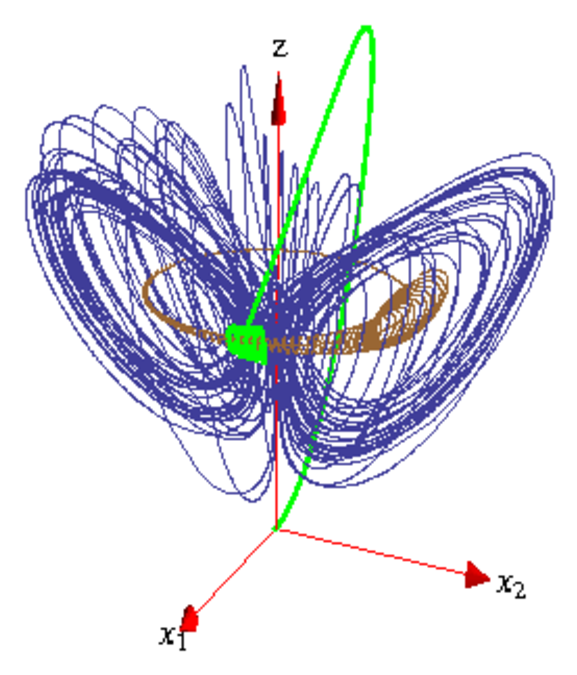
\includegraphics[height=0.25\textheight]{../figs/CLE}
\end{center}
\caption[Complex Lorenz flow phase space]
{ \Statesp\ portrait of \cLe\ dynamics for $e=1/10,\,
\ImrCLor=0$. Plotted are \reqv\ \REQV{}{1} (red), its unstable
manifold (brown), \eqv\ \EQV{0}, a representative of its
unstable manifold (green), 3 repetitions of \rpo\
``01''(magenta) and a generic orbit (blue).}
\label{fig:CLE}
\end{figure}
%%%%%%%%%%%%%%%%%%%%%%%%%%%%%%%%%%%%%%%%%%%%%%%%%%%%%%%%%%%%
%
\marginpar{Split: Fig1: reqb, generic trajectory, rpo. Fig2: reqb, unstable manifolds}

To find the location of the \reqv\ it is convenient to work
on polar coordinates defined by $x=r_1 e^{i \phi_1},\,y=r_2
e^{i \phi_2}$. Equations \refeq{eq:CLe} take the form
    %PC: Rebecca and I rederived these: they check.
\beq
\begin{split}
	\dot{r}_1 &=-\sigma (r_1 - r_2\cos\phi) \cont
	\dot{r}_2 &=-r_2 + r_1(\RerCLor -z)(\cos\phi-\ImrCLor\sin\phi) \cont
	\dot{z} &=  -b z+r_1 r_2\cos\phi \cont	
	\dot{\phi} &=-e-\frac{\sigma r_2 \sin\phi}{r_1}
             -\frac{r_1(\RerCLor-z) (\ImrCLor\cos\phi+\sin\phi) }{r_2}\,,
	\label{eq:CLePolar}
\end{split}
\eeq
where $\phi=\phi_1-\phi_2$ and the evolution equations for
$\phi_1,\phi_2$ are given by
\beq
\begin{split}
	\dot{\phi}_1 &=-\frac{\sigma r_2 \sin\phi}{r_1}\cont
	\dot{\phi_2} &= e +\frac{r_1\left(
         (\RerCLor -z)\sin\phi+\ImrCLor\cos\phi
                                \right)}{r_2}\,.
	\label{eq:CLeAngl}
\end{split}
\eeq

For simplicity we now turn to the ``laser case''
$e\neq0,\;\ImrCLor=0$. The condition for a \reqv\ is that all
time derivatives in \refeq{eq:CLePolar}, while
$\dot{\phi}_1=\dot{\phi}_2\neq 0$. If
$\dot{\phi}_1=\dot{\phi}_2=0$ we would have (a group orbit
of) equilibria. We get
\beq
\begin{split}
	z^{(1)} &= \frac{-e^2+(\RerCLor -1)(\sigma +1)^2}{(\sigma +1)^2}\cont
	r_1^{(1)} &= \sqrt{b z^{(1)}}\cont
	r_2^{(1)} &= \sqrt{b \left(e^2+(\sigma +1)^2\right)z^{(1)}}\cont
	\phi^{(1)} &= -\cos ^{-1}\left(\frac{\sigma +1}{\sqrt{e^2+(\sigma +1)^2}}\right)\,.
\end{split}
\eeq
Substituting in \refeq{eq:CLeAngl} we get
$\dot{\phi}_1=\dot{\phi}_2=e \sigma/(1 + \sigma)\neq 0$ for
$e\neq0$ and thus we have indeed a \reqv, not a group orbit
of \eqva.

Calculation  in polar coordinates $r_1,r_2,\phi,z$ of
stability eigenvalues for \REQV{}{1} for the set of
parameters we use here yields a weakly unstable spiral-out
\eqv\
\beq
	\eigRe[1]\pm i\eigIm[1]= 0.0938\pm 10.1945i,\,
    \eigExp[3]=-11.0009,\, \eigExp[4]= -13.8534\,.
	\label{eq:CLeREQBstab}
\eeq
In \ref{s:StabReq} we show how to calculate stability of
\reqva\ in \emph{equivariant} variables without change of
coordinates to polar or any other set of symmetry invariant
variables.


\section{\label{s:Hilbert} Symmetry reduction: Hilbert polynomial bases}
    \input symRedGeneral
    \input Hilbert

\section{\label{sec:mf} Symmetry reduction: Moving frames}
    \input movingFrames
    \input mfReqb
    \input mfLocal
    \input slice


\section{Conclusions}
    \input conclusions

\section*{Acknowledgements}
We are grateful to
D.~Barkley,
W.-J.~Beyn,
R.~Gilmore,
J.F.~Gibson,
J.~Halcrow,
K.A.~Mitchell,
C.W.~Rowley,
R.~Wilczak,
and in particular R.L.~Davidchack for many spirited exchanges.
P.C. thanks the
James Franck Institute, U. of Chicago,
for hospitality, and Argonne National Laboratory and
G.~Robinson Jr. for partial support.
E.S. was supported by NSF grant DMS-0807574 and G.~Robinson,~Jr.
%     \PC{
%     recheck initials for K. Mitchell,
%     }

% Specify following sections are appendices. Use \appendix* if there
% only one appendix.
\appendix

\section{\label{s:StabReq} Stability of \reqva}
    \input stabReqva

% \bibliographystyle{elsarticle-harv}
\bibliographystyle{elsarticle-num}
\bibliography{../bibtex/siminos}

\ifdraft
% remove this when all problems have been fixed
    \newpage
    \input 05fixMe
    \input flotsam
\fi
\end{document}
